%%% LaTeX-Vorlage Version 1.8 %%%

% Grundlegende Dokumenteneigenschaften gemäß DHBW-Vorgaben
\documentclass[a4paper,fontsize=11pt,oneside,parskip=half,headings=normal]{scrreprt} 
% \usepackage{showframe} % nur für Kontrolle der Ränder 

%%% Präambel einbinden (mit Festlegungen gemäß DHBW-Vorgaben) %%%
%%% Präambel %%%
% hier sollten keine Änderungen erforderlich sein
%
\usepackage[utf8]{inputenc}   % Zeichencodierung UTF-8 für Eingabe-Dateien
\usepackage[T1]{fontenc}      % Darstellung von Umlauten im PDF

\usepackage{listings}         % für Einbindung von Code-Listings
\lstset{numbers=left,numberstyle=\tiny,numbersep=5pt,texcl=true}
\lstset{literate=             % erlaubt Sonderzeichen in Code-Listings 
{Ö}{{\"O}}1
{Ä}{{\"A}}1
{Ü}{{\"U}}1
{ß}{{\ss}}2
{ü}{{\"u}}1
{ä}{{\"a}}1
{ö}{{\"o}}1
{€}{{\euro}}1
}

\usepackage[
  inner=35mm,outer=15mm,top=25mm,
  bottom=20mm,foot=12mm,includefoot
]{geometry}                 % Einstellungen für Ränder

\usepackage[english]{babel} % Spracheinstellungen Englisch
\usepackage[babel,english=british]{csquotes} % englische Anf.zeichen
\usepackage{enumerate}      % anpassbare Nummerier./Aufz.
\usepackage{graphicx}       % Einbinden von Grafiken
\usepackage[onehalfspacing]{setspace} % anderthalbzeilig

\usepackage{blindtext}      % Textgenerierung für Testzwecke
\usepackage{color}          % Verwendung von Farbe 

\usepackage{acronym}        % für ein Abkürzungsverzeichnis

\usepackage[                % Biblatex
  backend=biber,
  bibstyle=_dhbw_authoryear,maxbibnames=99,
  citestyle=authoryear,     
  uniquename=true, useprefix=true,
  bibencoding=utf8]{biblatex}
%kein Punkt am Ende bei \footcite
%http://www.golatex.de/footcite-ohne-punkt-am-schluss-t4865.html
\renewcommand{\bibfootnotewrapper}[1]{\bibsentence#1}


%Reihenfolge der Autorennamen
%   
% http://golatex.de/viewtopic,p,80448.html#80448
% Argumente: siehe http://texwelt.de/blog/modifizieren-eines-biblatex-stils/
\DeclareNameFormat{sortname}{% Bibliographie
  \ifnum\value{uniquename}=0 % Normalfall
    \ifuseprefix%
      {%
         \usebibmacro{name:family-given}
           {\namepartfamily}
           {\namepartgiveni}
           {\namepartprefix}
           {\namepartsuffixi}%
       }
      {%
         \usebibmacro{name:family-given}
           {\namepartfamily}
           {\namepartgiveni}
           {\namepartprefixi}
           {\namepartsuffixi}%
       }%
  \fi
  \ifnum\value{uniquename}=1% falls nicht eindeutig, abgek. Vorname 
      {%
         \usebibmacro{name:family-given}
           {\namepartfamily}
           {\namepartgiveni}
           {\namepartprefix}
           {\namepartsuffix}%
       }%
  \fi
  \ifnum\value{uniquename}=2% falls nicht eindeutig, ganzer Vorname 
      {%
         \usebibmacro{name:family-given}
           {\namepartfamily}
           {\namepartgiven}
           {\namepartprefix}
           {\namepartsuffix}%
       }%
  \fi   
  \usebibmacro{name:andothers}}

\DeclareNameFormat{labelname}{% für Zitate
  \ifnum\value{uniquename}=0 % Normalfall
    \ifuseprefix%
      {%
         \usebibmacro{name:family-given}
           {\namepartfamily}
           {\empty}
           {\namepartprefix}
           {\namepartsuffixi}%
       }
      {%
         \usebibmacro{name:family-given}
           {\namepartfamily}
           {\empty}
           {\namepartprefixi}
           {\namepartsuffixi}%
       }%
  \fi
  \ifnum\value{uniquename}=1% falls nicht eindeutig, abgek. Vorname 
      {%
         \usebibmacro{name:family-given}
           {\namepartfamily}
           {\namepartgiveni}
           {\namepartprefix}
           {\namepartsuffix}%
       }%
  \fi
  \ifnum\value{uniquename}=2% falls nicht eindeutig, ganzer Vorname 
      {%
         \usebibmacro{name:family-given}
           {\namepartfamily}
           {\namepartgiven}
           {\namepartprefix}
           {\namepartsuffix}%
       }%
  \fi   
  \usebibmacro{name:andothers}}
      
  
\DeclareFieldFormat{extrayear}{% = the 'a' in 'Jones 1995a'
  \iffieldnums{labelyear}
    {\mknumalph{#1}}
    {\mknumalph{#1}}}        

\renewcommand*{\multinamedelim}{\addslash}
\renewcommand*{\finalnamedelim}{\addslash}
\renewcommand*{\multilistdelim}{\addslash}
\renewcommand*{\finallistdelim}{\addslash}

\renewcommand{\nameyeardelim}{~}

% Literaturverzeichnis: Doppelpunkt zwischen Name (Jahr): Rest 
% http://de.comp.text.tex.narkive.com/Tn1HUIXB/biblatex-authoryear-und-doppelpunkt
\renewcommand{\labelnamepunct}{\addcolon\addspace}

% damit die Darstellung für Vollzitate von Primärquellen in 
% Fußnoten später auf "nicht fett" geändert werden kann 
% (nur für Zitate von Sekundärliteratur relevant)
\newcommand{\textfett}[1]{\textbf{#1}}

% für Zitate von Sekundärliteratur:
\newcommand{\footcitePrimaerSekundaer}[4]{%
  \renewcommand{\textfett}[1]{##1}%
  \footnote{\fullcite[#2]{#1}, zitiert nach \cite[#4]{#3}}%  
  \renewcommand{\textfett}[1]{\textbf{##1}}%
}

% Im Literaturverzeichnis: Autor (Jahr) fett
\renewbibmacro*{author}{%
  \ifboolexpr{%
    test \ifuseauthor%
    and
    not test {\ifnameundef{author}}
  }
    {\usebibmacro{bbx:dashcheck}
       {\bibnamedash}
       {\usebibmacro{bbx:savehash}%
        \textfett{\printnames{author}}%
        \iffieldundef{authortype}
          {\setunit{\addspace}}
          {\setunit{\addcomma\space}}}%
     \iffieldundef{authortype}
       {}
       {\usebibmacro{authorstrg}%
        \setunit{\addspace}}}%
    {\global\undef\bbx@lasthash
     \usebibmacro{labeltitle}%
     \setunit*{\addspace}}%
  \textfett{\usebibmacro{date+extrayear}}}

% Sonderfall: Quelle ohne Autor, aber mit Herausgeber
% Name des Herausgebers wird fett gedruckt
\renewbibmacro*{bbx:editor}[1]{%
  \ifboolexpr{%
    test \ifuseeditor%
    and
    not test {\ifnameundef{editor}}
  }
    {\usebibmacro{bbx:dashcheck}
       {\bibnamedash}
       {\textfett{\printnames{editor}}%
        \setunit{\addcomma\space}%
        \usebibmacro{bbx:savehash}}%
     \usebibmacro{#1}%
     \clearname{editor}%
     \setunit{\addspace}}%
    {\global\undef\bbx@lasthash
     \usebibmacro{labeltitle}%
     \setunit*{\addspace}}%
  \textfett{\usebibmacro{date+extrayear}}}

% Anpassungen für deutsche Sprache
\DefineBibliographyStrings{ngerman}{%
	nodate = {{o.J.}},
	urlseen = {{Abruf:}},
	ibidem = {{ebenda}}
}

% keine Anführungszeichen beim Titel im Literaturverzeichnis
\DeclareFieldFormat[article,book,inbook,inproceedings,manual,misc,phdthesis,thesis,online,report]{title}{#1\isdot}

\newcommand{\literaturverzeichnis}{%
% nur Literaturverzeichnis
% (als eigenes Kapitel)
\phantomsection
\addcontentsline{toc}{chapter}{Literaturverzeichnis}
\spezialkopfzeile{Literaturverzeichnis}
\defbibheading{lit}{\chapter*{Literaturverzeichnis}}
\label{chapter:quellen}
\printbibliography[heading=lit,notkeyword=ausblenden]
} % mit DHBW-spezifischen Einstellungen

\usepackage{hyperref}       % URL-Formatierung, klickbare Verweise

\usepackage{tocloft}        % für Verzeichnis der Anhänge

\newcounter{anhcnt}
\setcounter{anhcnt}{0}
\newlistof{anhang}{app}{}

\newcommand{\anhang}[1]{%
  \refstepcounter{anhcnt}
  \setcounter{anhteilcnt}{0}
  \section*{Appendix \theanhcnt: #1}
  \addcontentsline{app}{section}{\protect\numberline{Anhang \theanhcnt}#1}\par
}

\newcounter{anhteilcnt}
\setcounter{anhteilcnt}{0}

\newcommand{\anhangteil}[1]{%
	\refstepcounter{anhteilcnt}
	\subsection*{Anhang~\arabic{anhcnt}/\arabic{anhteilcnt}: #1}
	\addcontentsline{app}{subsection}{\protect\numberline{Anhang \theanhcnt/\arabic{anhteilcnt}}#1}\par
}

\renewcommand{\theanhteilcnt}{Anhang \theanhcnt/\arabic{anhteilcnt}}

% vgl. S. 4 Paket-Beschreibung tocloft 	
% Einrückungen für Anhangverzeichnis
\makeatletter
\newcommand{\abstaendeanhangverzeichnis}{
\renewcommand*{\l@section}{\@dottedtocline{1}{0em}{5.5em}}
\renewcommand*{\l@subsection}{\@dottedtocline{2}{2.3em}{6.5em}}
}
\makeatother

% Abbildungs- und Tabellenverzeichnis
% Bezeichnungen
% \renewcaptionname{ngerman}{\figurename}{Abb.}
% \renewcaptionname{ngerman}{\tablename}{Tab.}
% Einrückungen
\makeatletter
\renewcommand*{\l@figure}{\@dottedtocline{1}{0em}{2.3em}}
\renewcommand*{\l@table}{\@dottedtocline{1}{0em}{2.3em}}
\makeatother


\usepackage{chngcntr}                % fortlaufende Zähler für Fußnoten, Abbildungen und Tabellen
\counterwithout{figure}{chapter}
\counterwithout{table}{chapter}
\counterwithout{footnote}{chapter}

\usepackage[automark]{scrlayer-scrpage} 
%% Definitionen für Kopf- und Fußzeile auf normalen Seiten
\defpagestyle{kopfzeile}
{% Kopfdefinition
  (\textwidth,0pt)    % Länge der oberen Linie,Dicke der oberen Linie       
  {} % Definition für linke Seiten im doppelseitigen Layout
  {} % Definition für rechte Seiten im doppelseitigen Layout      
  {  % Definition für Seiten im einseitigen Layout
	\makebox[0pt][l]{\rightmark}% 
	\makebox[\linewidth]{}% 
  }        
  (\textwidth, 0.4pt) % Untere Linienlänge, Untere Liniendicke
}
{% Fußdefinition
  (\textwidth,0pt)    % Obere Linienlänge, Obere Liniendicke
  {} % Definition für linke Seiten im doppelseitigen Layout
  {} % Definition für rechte Seiten im doppelseitigen Layout
  {  % Definition für Seiten im einseitigen Layout
    \makebox[\linewidth]{}%
    \makebox[0pt][r]{\pagemark}%
  }
  (\textwidth, 0pt)   % Länge der unteren Linie,Dicke der unteren Linie
}

%% Definitionen für Kopf- und Fußzeile auf ersten Seiten eines Kapitels
\defpagestyle{kapitelkopfzeile}
{% Kopfdefinition
  (\textwidth,0pt)    % Länge der oberen Linie,Dicke der oberen Linie       
  {} % Definition für linke Seiten im doppelseitigen Layout
  {} % Definition für rechte Seiten im doppelseitigen Layout      
  {}  % Definition für Seiten im einseitigen Layout
  (\textwidth, 0pt) % Untere Linienlänge, Untere Liniendicke
}
{% Fußdefinition
  (\textwidth,0pt)    % Obere Linienlänge, Obere Liniendicke
  {} % Definition für linke Seiten im doppelseitigen Layout
  {} % Definition für rechte Seiten im doppelseitigen Layout
  {  % Definition für Seiten im einseitigen Layout
    \makebox[\linewidth]{}%
    \makebox[0pt][r]{\pagemark}%
  }
  (\textwidth, 0pt)   % Länge der unteren Linie,Dicke der unteren Linie
}

%% Definitionen für Kopf- und Fußzeile im Anhang und bei Quellenverzeichnisse
\newcommand{\spezialkopfzeileBezeichnung}{}
\defpagestyle{spezialkopfzeile}
{% Kopfdefinition
  (\textwidth,0pt)    % Länge der oberen Linie,Dicke der oberen Linie       
  {} % Definition für linke Seiten im doppelseitigen Layout
  {} % Definition für rechte Seiten im doppelseitigen Layout      
  {  % Definition für Seiten im einseitigen Layout
	\makebox[0pt][l]{\spezialkopfzeileBezeichnung}% 
	\makebox[\linewidth]{}% 
  }        
  (\textwidth, 0.4pt) % Untere Linienlänge, Untere Liniendicke
}
{% Fußdefinition
  (\textwidth,0pt)    % Obere Linienlänge, Obere Liniendicke
  {} % Definition für linke Seiten im doppelseitigen Layout
  {} % Definition für rechte Seiten im doppelseitigen Layout
  {  % Definition für Seiten im einseitigen Layout
    \makebox[\linewidth]{}%
    \makebox[0pt][r]{\pagemark}%
  }
  (\textwidth, 0pt)   % Länge der unteren Linie,Dicke der unteren Linie
}
            
\newcommand\spezialkopfzeile[1]{%
  \renewcommand\spezialkopfzeileBezeichnung{#1}
  \pagestyle{spezialkopfzeile}
}
                
% Standard-Pagestyle auswählen
\pagestyle{kopfzeile}

% keine Kopfzeile anzeigen auf Seiten, auf denen ein 
% Kapitel beginnt oder das Inhalts-/Abbildungs-/Tabellenverzeichnis steht 
\renewcommand{\chapterpagestyle}{kapitelkopfzeile}
\tocloftpagestyle{kapitelkopfzeile}

		 % für schöne Kopfzeilen 

\usepackage{textcomp}            % erlaubt EUR-Zeichen in Eingabedatei
\usepackage{eurosym}             % offizielles EUR-Symbol in Ausgabe
\renewcommand{\texteuro}{\euro}  % ACHTUNG: nach hyperref aufrufen!

\usepackage{scrhack}             % stellt Kompatibilität zw. KOMA-Script
                                 % (scrreprt) und anderen Paketen her
                                 
% Anpassung der Abstände bei Kapitelüberschriften
% (betrifft auch Inhalts-, Abbildungs- und Tabellenverzeichnis)
\renewcommand*\chapterheadstartvskip{\vspace*{-\topskip}}
\newcommand{\myBeforeTitleSkip}{1mm}
\newcommand{\myAfterTitleSkip}{10mm}
\setlength\cftbeforetoctitleskip{\myBeforeTitleSkip}
\setlength\cftbeforeloftitleskip{\myBeforeTitleSkip}
\setlength\cftbeforelottitleskip{\myBeforeTitleSkip}

\setlength\cftaftertoctitleskip{\myAfterTitleSkip}
\setlength\cftafterloftitleskip{\myAfterTitleSkip}
\setlength\cftafterlottitleskip{\myAfterTitleSkip}                                                            
%%% Ende der Präambel %%%

%%% Name der eigenen Literatur-Datenbank (ggf. anpassen) %%%
\bibliography{includes/literatur-datenbank.bib}

\begin{document}
%%% Deckblatt einbinden %%% 
% Anpassungen nötig (Name, Titel etc.)
% HIER EDITIEREN: 
% Typ der Arbeit (für Deckblatt und ehrenwörtliche Erklärung)
% - bitte Zutreffendes auswählen
%\newcommand{\typMeinerArbeit}{1. Projektarbeit} 
%\newcommand{\typMeinerArbeit}{2. Projektarbeit} 
%\newcommand{\typMeinerArbeit}{Seminararbeit} 
\newcommand{\typMeinerArbeit}{Project Thesis} 

% Thema der Arbeit (für ehrenwörtliche Erklärung, ohne Umbrüche)
% HIER EDITIEREN: 
\newcommand{\themaMeinerArbeit}{Mein Titel}

% Vorname, Name der Autorin/des Autors (für Titelseite und Metadaten)
% HIER EDITIEREN:
\newcommand{\meinName}{Tim Struthoff}

\thispagestyle{empty}

\begin{spacing}{1}
\begin{center}	
~\vspace{0mm}

% HIER EDITIEREN: Titel der Arbeit
{\sffamily
\LARGE  
% \Large  % bei sehr langen Titeln ggf. etwas kleinere Schriftart wählen
\textbf{Titel der Arbeit}

\bigskip
\textbf{ggf. etwas länger}
}


\vspace{15mm}

% Typ wird automatisch eingefügt (oben festlegen)
{\Large \typMeinerArbeit}

\vspace{1cm}

% HIER ggf. EDITIEREN
vorgelegt am \today 

\vspace{15mm}

Fakultät Wirtschaft
\medskip

Studiengang Wirtschaftsinformatik
\medskip

% HIER EDITIEREN: Kurs eintragen
Kurs ... 

\vspace{10mm}

von

\vspace{10mm}

% Vorname und Name wird automatisch eingefügt (oben festlegen) 
{\large\textsc{\meinName}}

\vspace{10mm}
\end{center}

\vfill

% HIER EDITIEREN: Name des Unternehmens, Name der Betreuerin/des Betreuers
\begin{tabular}{ll}
Betreuer in der Ausbildungsstätte: & DHBW Stuttgart: \\
\hspace{0.4\linewidth} & \\
$\langle$ Hewlett Packard Enterprise Company $\rangle$ & $\langle$ Titel, Vorname und Nachname $\rangle$ \\
$\langle$ Titel, Vorname und Nachname der Betreuerin $\rangle$ 
& $\langle$ der/des wissenschaftlichen Betreuerin/Prüferin $\rangle$ \\
$\langle$ Funktion der Betreuerin/des Betreuers $\rangle$ \\
\\
Unterschrift der Betreuerin/des Betreuers \\
\end{tabular}


\vspace{1cm}
%(etwas Platz für die Unterschrift der Betreuerin/des Betreuers aus der Ausbildungsstätte)
\end{spacing}

% falls ein Vertraulichkeitsvermerk erforderlich ist,
% die Kommentarzeichen in den nachfolgenden Zeilen entfernen:
 
%\begin{center}
%\small
%\textbf{Vertraulichkeitsvermerk}:
%Der Inhalt dieser Arbeit darf weder als Ganzes noch in Auszügen \\
%Personen außerhalb des Prüfungs- und Evaluationsverfahrens zugänglich gemacht werden, sofern keine anders lautende Genehmigung des Dualen Partners vorliegt. 
%\end{center}

% Meta-Daten für PDF-Datei basierend auf obigen Angaben
\hypersetup{pdftitle={\themaMeinerArbeit}}
\hypersetup{pdfauthor={\meinName}}
\hypersetup{pdfsubject={\typMeinerArbeit\ DHBW Stuttgart \the\year}}

%%% Umstellung der Seiten-Nummerierung auf i, ii, iii ... %%%
\pagenumbering{Roman} 

%%% Abstract einbinden (optionale Kurzfassung Ihrer Arbeit) %%%
\begin{abstract}
\thispagestyle{kapitelkopfzeile}
\textbf{Title of the abstract}

This is going to be the abstract


\end{abstract}


\cleardoublepage

%%% Inhalts-, Abbildungs-, Tabellenverzeichnisse %%%
% sollen einzeilig gesetzt werden, um Platz zu sparen 
\begin{spacing}{1}
\tableofcontents
\clearpage
\chapter*{Appendix}
\addcontentsline{toc}{chapter}{Appendix}
\section*{List of appendices}

\begin{acronym}[DHBW] 
% Argument definiert die Breite der ersten Spalte anhand des längsten vorkommenden Eintrags
\acro{CRM}{Customer Relationship Management}
\end{acronym}

\vspace{2em}

\clearpage
\thispagestyle{kapitelkopfzeile}
\listoffigures
\phantomsection
\addcontentsline{toc}{chapter}{Abbildungsverzeichnis} % Abb.verz. ins Inh.verz. aufnehmen

\clearpage
\listoftables
\phantomsection
\addcontentsline{toc}{chapter}{Tabellenverzeichnis}   % Tab.verz. ins Inh.verz. aufnehmen
\end{spacing}

%%% Umstellung der Seiten-Nummerierung auf 1, 2, 3 ... %%%
\cleardoublepage
\pagenumbering{arabic}

%%% Ihr eigentlicher Inhalt %%%
% Empfehlung: strukturieren Sie Ihren Text in einzelnen Dateien 
% und binden Sie diese hier mit \input{includes/dateiname.tex} ein

\chapter{Einleitung}\label{chapter:einleitung}

Die Hewlett Packard Enterprise (HPE) Business Unit Aruba Networks bietet neben anderen Netzwerkgeräten auch Wireless Local Area Network (WLAN) Zugangspunkte bzw. Access Points (APs) an. Mit diesen Zugangspunkten ist es möglich, Endgeräte drahtlos an ein Netzwerk anzubinden\footcite[Vgl. ][]{hewlett_packard_enterprise_development_lp_access_2021}. Ein Kunde der Aruba Networks setzt mehrere hundert dieser APs ein. Er verwaltet alle seine IT Geräte, also auch die Aruba APs, mit einer Inventarisierungssoftware. Mit dieser Software sollen nun periodisch Inventardaten zu den APs abgerufen werden. Zur Einsparung von Arbeitskosten soll das Abrufen dieser Daten automatisiert werden. Die Aruba APs werden zentral über den SNMP basierten cloud-managed Service Aruba Central Cloud verwaltet. Die Aruba Central Cloud stellt eine sog. Representational State Transfer (REST) Schnittstelle zur Verfügung, über die Statusdaten der APs abgerufen werden können. Ein JavaScript Programm soll sich nun mit der Aruba REST Schnittstelle verbinden und so die Statusdaten der APs automatisiert abrufen. Somit fungiert das in dieser Arbeit konzipierte Programm als eine Middleware zwischen Aruba Cloud Central und der Inventarisierungssoftware des Kunden. 

\section{Zielsetzung}\label{section:zielsetzung}

Das betriebliche, praktische Ziel dieser Arbeit stellt die Umsetzung eines Prototyps für die zuvor gezeigte Middleware dar. Das theoretische, bzw. akademische Ziel dieser Arbeit liegt in der formalisierten Aufbereitung des Recherche- und Implementierungsprozesses für die Interaktion der Middleware mit der REST API. Konkret sollen folgende \textbf{Forschungsfragen} beantwortet werden:

\begin{enumerate}
    \item Wie ist der Representational State Transfer Architekturstil von Roy Fielding aufgebaut?
    \item Wie kann überprüft werden, ob eine API den REST Prinzipien entspricht?
    \item Entspricht die API der Managementsoftware Aruba Cloud Central den Grundsätzen von Roy Fieldings REST Architektur und werden auch andere Empfehlungen aus Fachliteratur beachtet?
    \item Kann sich ein JavaScript Programm mit der Aruba Schnittstelle verbinden und mittels REST HTTP Abfragen Informationen über Aruba Geräte in der Netzwerkumgebung des Kunden sammeln?
\end{enumerate}

Zusammengefasst liegt das Ziel der Arbeit in der Aufbereitung, Analyse und examplarischen Anwendung des REST Architekturstils am Beispiel der Aruba Central API.

\section{Verwandte Arbeiten}\label{section:verwandte-arbeiten}

Zu dem REST Architekturstil wurden bereits zahlreiche Arbeiten veröffentlicht. Speziell der Analyse von REST APIs haben sich die folgenden Autoren gewidmet. Bei allen unten aufgeführten Werken lag der Fokus jedoch nicht auf einer speziellen API oder gar einem Endpunkt, sondern in der Analyse einer Vielzahl von APIs.

\begin{itemize}
    \item \textbf{Renzel et. al} untersuchen in einer Arbeit von 2012 eine Reihe von populären REST Webservices hinsichtlich ihrer Konformität mit Best Practices\footcite[Vgl. ][]{hutchison_todays_2012}.

    \item \textbf{Maleshkova et. al} analysieren die Dokumentation von 222 APIs und ziehen Rückschlüsse auf gängige Beschreibungsformen, Ausgabetypen, die Verwendung von API-Parametern sowie weiteren Merkmalen\footcite[Vgl. ][]{maleshkova_investigating_2010}. In einer anderen Arbeit werden von Maleshkova 45 APIs von der Website ProgrammableWeb analysiert\footcite[Vgl. ][]{presutti_restful_2014}. 

    \item \textbf{Neumann et al} sammelt Regeln zum Aufbau von REST APIs und analysiert 500 APIs der Alexa.com 4000 populärsten Websites. Neumann et al referenzieren in der Auswahl der Best Practices Renzel, Maleshkova 2014 und Rodriguez et. al 2016.

    \item In \textbf{Rodriguez et al 2016} wurden 78 GB internet traffic der Telecom Italia analysiert. Die Autoren stellen einige Regeln für REST APIs zusammen und analysieren den Traffic hinsichtlich der Konformität mit diesen Regeln\footcite[Vgl. ][]{rodriguez_rest_2016}. 

\end{itemize}

\section{Forschungsbeitrag}\label{section:forschungsbeitrag}

Der akademische Mehrwert dieser Arbeit begründet sich aus dem Zusammenstellen von konkreten Handlungsrichtlinien zur Implementierung von REST APIs aus vorhandener Literatur und der exemplarischen Anwendung dieser Regeln auf die Aruba Central API. Durch die exemplarische Anwendung dieses heuristischen Regelwerks wird das Regelwerk einerseits validiert und andererseits ein Beispiel gegeben, welches es zukünftigen Anwendern ermöglicht, die Regeln besser anzuwenden. Abschließend wird die Relevanz der Regeln mit einem Prototyp validiert. Zusammengefasst ist es Lesern dieser Arbeit möglich, REST APIs zu klassifizieren und auf Basis dieser Einordnung eine Entscheidung zu der Machbarkeit der Implementierung von Software mit der API zu treffen. Auch ist die Arbeit als firmeninternes Referenzwerk gedacht.

In der Problemdomäne ist bereits eine Vielzahl an Regelwerken zu REST APIs vorhanden. Diese Arbeit unterscheidet sich jedoch von vorhandener Literatur in ihrer Spezifität zu dem betrieblichen Kontext der Aruba Networks, sowie der Validierung der Forschungsergebnisse mittels eines Prototyps.

Neben der positiven Eingrenzung des Themenbereichs dieser Arbeit muss auch eine negative Abgrenzung stattfinden: Der Fokus dieser Arbeit liegt allein auf dem REST Architekturstil mit der konkreten Anwendung im HTTP Protokoll. Es werden keine alternativen Architekturstile in Betracht gezogen. Auch können die, in dieser Arbeit gewonnenen Ergebnisse nicht als absolute, unlimitiert gültige Wahrheit gesehen werden. Die Umsetzung des REST Stils entwickelt sich dynamisch und ist weitgehend frei von regulatorischer Kontrolle. So können die hier erlangten Ergebnisse lediglich als eine Heuristik auf Basis von aktueller, verbreiteter Literatur und etablierter Unternehmenspraxis gesehen werden. Eine weitere Einschränkung der Arbeit liegt in der Analyse von lediglich einem Endpunkt der Aruba Central API. Zwar ist anzunehmen, dass alle anderen Endpunkte der API ähnlich zu dem hier analysierten sind, jedoch kann dies aufgrund des beschränkten Umfangs der Arbeit nicht validiert werden. Zusätzlich liegt der Fokus bei der Umsetzung des Prototyps nicht auf konkreten Implementierungsdetails sondern auf dem Beweis der Machbarkeit einer Integration mit der Aruba Central API.


\section{Aufbau der Arbeit}\label{section:aufbau-der-arbeit}

Zunächst wird das Thema in Kapitel \ref{chapter:theoretische-betrachtung} aus theoretischer Sicht beleuchtet. Zur Beantwortung der ersten Forschungsfrage nach dem Aufbau einer REST API wird in Kapitel \ref{section:quellendiskussion} vorhandene Fachliteratur ausgewählt und die Auswahl begründet. In Kapitel \ref{subsection:definitionen-und-begriffe} wird ein Grundwortschatz aus Fachbegriffen vorgestellt. Auf diesen Wortschatz wird in der weiteren Arbeit zurückgegriffen. Weiter wird in Kapitel \ref{subsection:der-rest-architekturstil} der REST Architekturstil in seiner Ausführung von Fielding erläutert. Zur späteren Klassifizierung der Aruba Central REST API wird in Kapitel \ref{section:klassifizierung-von-rest} ein Gütemodell von Richardson um weitere Quellen erweitert und so ein Referenzmodell geschaffen.

Im Praxisteil (Kapitel \ref{chapter:praxisteil}) der Arbeit werden die erlangten Erkenntnisse angewendet und so validiert. Zunächst wird die betriebliche Problemstellung erläutert (Kapitel \ref{section:problemstellung-der-betrieblichen-praxis}). Dann wird der Aruba Central Monitoring Endpunkt analysiert (Kapitel \ref{section:analyse-des-access-point-monitoring-endpunkte}) und in das in Kapitel \ref{section:klassifizierung-von-rest} erstellte Referenzmodell eingeordnet. Diese Einordnung soll eine grobe Einschätzung der Machbarkeit des Middleware Programmes ermöglichen. Das Analyseergebnis wird in Kapitel \ref{section:Evaluierung-des-Analyseergebnisses-durch-Prototyping} mittels eines Prototyps validiert: Wurde die API in Kapitel \ref{section:analyse-des-access-point-monitoring-endpunkte} als RESTful eingestuft, sollte die Umsetzung des Prototyps möglich sein.

Im Fazit der Arbeit werden die erlangten Forschungsergebnisse zusammengefasst (Kapitel \ref{chapter:fazit}) und kritisch hinterfragt (Kapitel \ref{section:kritische-Evaluierung}). Abschließend wird in Kapitel \ref{section:ausblick} ein Ausblick auf weitere Entwicklungen der Arbeit gegeben.





\chapter{Theoretische Betrachtung des REST Architekturstils}\label{chapter:theoretische-betrachtung}

Bei der Umsetzung einer Middleware zur REST Kommunikation stellt sich zunächst die erste Forschungsfrage nach dem Aufbau einer solchen REST Kommunikation. Der REST Architekturstil wird im Folgenden aus der Primärliteratur von Roy Fielding sowie anderer Fachliteratur herausgearbeitet und abstrahiert zusammengefasst:

\section{Quellendiskussion}\label{section:quellendiskussion}

Der REST Architekturstil wurde von Roy Fielding erfunden und zuerst in Fieldings Doktorarbeit “Architectural Styles and the Design of Network-based Software Architectures” beschrieben. Somit kann die Dissertation von Fielding als erste und wichtigste Primärquelle angesehen werden. Der REST Architekturstil ist eine Abstraktion des ebenfalls zu großen Teilen von Fielding konzipierten HTTP Protokolls . Somit sollte das HTTP Protokoll in der Fassung von 1999 auch als Primärquelle aufgenommen werden. Auch andere Request For Comments (RFC) der IETF werden als Primärquelle angesehen. 

Die Arbeit von Fielding befasst sich nicht mit der Umsetzung der Regel des REST Stils und auch nicht mit der Priorisierung dieser Regeln. Diese beiden Aspekte werden jedoch für diese Arbeit benötigt. Für diese Informationen wird auf Sekundärliteratur zurückgegriffen. 

\subsection{Quellen zur konkreten Umsetzung des REST Architekturstils}\label{subsection:qullen-zur-konkreten-umsetzung}

\begin{figure}[htb]
\centering
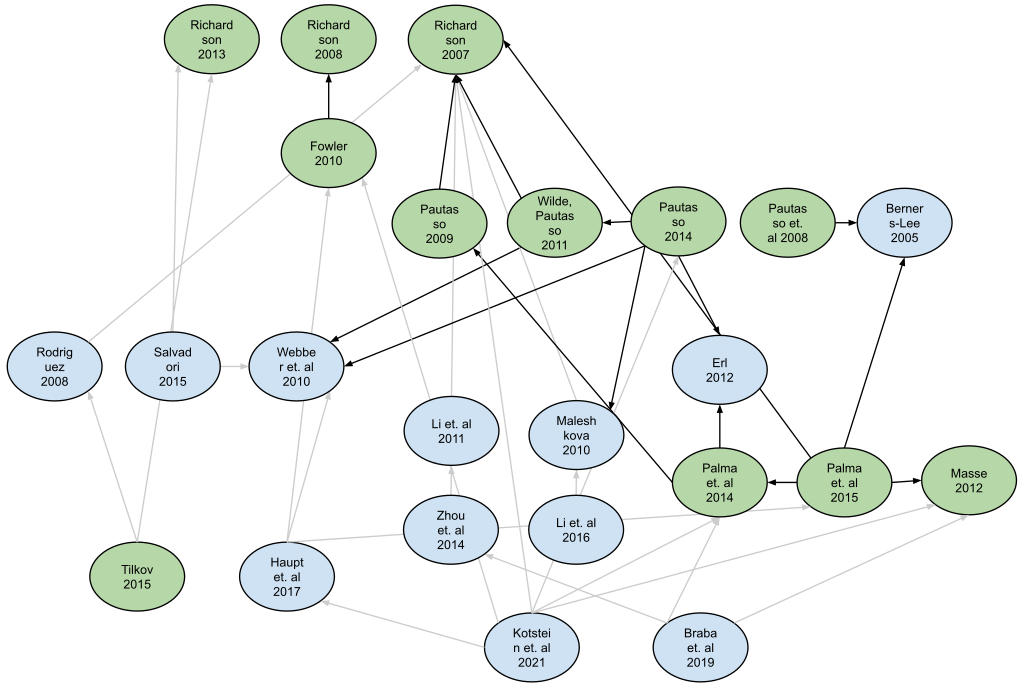
\includegraphics[width=\textwidth]{graphics/quelleneinordnung.png}
\caption[quelleneinordnung]{Quelleneinordnung}
\label{abb:QuellenEinordnung}
\end{figure}


Es wurde eine Vielzahl von Quellen untersucht. Diese Quellen sind in Abbildung .. aufgeführt. 

Die Kreise stellen die einzelnen Quellen dar. Ein Pfeil von Quelle A zu Quelle B symbolisiert eine Referenz von Quelle A auf Quelle B. Alle Quellen beziehen sich zusätzlich zu den hier aufgeführten Referenzen auf Roy Fieldings Doktorarbeit. Zur weiteren Synthese der Quellen wurde versucht, die Qualität der Quellen zu beurteilen. Alle als qualitativ beurteilten Quellen sind in der Abbildung in grün dargestellt. Diese werden in der folgenden Arbeit hauptsächlich verwendet. Die Beurteilung der Quellen wird im Folgenden begründet:

Zunächst werden die Quellen von Richardson von 2007, 2008 und 2013 betrachtet: Alle Quellen werden vielfach zitiert. Da andere Autoren ebenfalls auf die Auswahl hochwertiger Quellen achten sollten, lässt sich annehmen, dass eine viel zitierte Quelle von hoher Qualität ist. Gerade das Lehrbuch “RESTful Web Services” (2007) wurde besonders oft zitiert. Zusätzlich sind Richardsons Werke bei dem 1978 gegründeten, anerkannten Verleger O’Reilly publiziert. Weitergehend ist Leonard Richardson der Autor der populären  Bibliothek Beautiful Soup zum parsen von XML und HTML Dokumenten  und arbeitete bereits als Software Architekt bei der New York Public Library, sowie bei Canonical, der Firma hinter Ubuntu. Insgesamt wurden seine Werke über 1500 mal zitiert.

Auch die Werke von Pautasso wurden vielfach zitiert. Cesare Pautasso is full professor at the Software Institute of the Faculty of Informatics at the University of Lugano, Switzerland. Previously he was a researcher at the IBM Zurich Research Lab (2007) and a senior researcher at ETH Zurich (2004-2007). He completed his graduate studies with a Ph.D. from ETH Zurich in 2004 and his undergraduate studies at Politecnico di Milano, Italy with a Computer Science Engineering Degree (cum laude) in 2000.

Francis Palma wird ebenfalls als ein Spezialist auf seinem Fachgebiet angesehen und weißt einen h-Index von 12 auf. Seine Werke werden unter kritischer Betrachtung ebenfalls als Quellen aufgenommen.

Ein Lehrbuch von Mark Masse wird auch als Quelle aufgenommen. Masse verfügt über fünfzehn Jahre Erfahrung in Technik, Management und Architektur der Informatik und entwarf das Content Management System (CMS) von allen Websites der Walt Disney Company. Das vorliegende Lehrbuch ist jedoch teils subjektiv gehalten und sollte somit besonders kritisch hinterfragt werden.

Eine weitere betrachtete Quelle ist ein Lehrbuch von Stefan Tilkov. Das Lehrbuch wurde aufgrund einer mündlichen Empfehlung der Bibliothek der Dualen Hochschule Baden-Württemberg (DHBW) sowie der Universität Stuttgart ausgewählt. Auch ist Stefan Tilkov Berater bei INNOQ, Autor zahlreicher Fachartikel und Referent auf zahlreichen internationalen Konferenzen. Gleichzeitig wurde das Buch jedoch laut Google Scholar nur 15 mal zitiert. Aus diesem Grund wird es im Folgenden auch kritischer betrachtet.

\subsection{Quellen zur Priorisierung der Rest Regeln}\label{subsection:quellen-zur-priorisierung}

Johanna Barzen und Sebastian Kotstein erstellten eine Umfrage unter Experten, welche REST Regeln am wichtigsten sind. Die Meinungen dieser Experten werden auch in der Priorisierung der REST Regeln in dieser Arbeit berücksichtigt.

\section{Definitionen und Begriffe}\label{subsection:definitionen-und-begriffe}

Fielding legte bei der formulierung seines REST Architekturstil einen besonderen Fokus auf die Definition und korrekte Verwendung von speziellen Begriffen. Diese werden im folgenden zusammengefasst.

\subsection{Ressourcen und Repräsentationen}\label{subsection:ressourcen-und-repraesentationen}

Da es sich bei REST um einen Stil zur Umsetzung von verteilten Informationssystemen handelt, liegt es auf der Hand, zunächst die Modellierung von Informationen zu betrachten. Die Abstraktion einer jeden Information in REST stellt eine Ressource dar . Zu jedem Abfragezeitpunkt entspricht eine Ressource einem bestimmten Set von Ressourcen Repräsentationen und/-oder Ressourcen Metadaten. Ressourcen Repräsentationen sind konkrete Daten in einer konkreten Darstellungsform, wie zum Beispiel ein Bild oder ein Text  . Die Metadaten beschreiben diese Daten, sodass sie angemessen verarbeitet werden können.

\subsection{Verbindungselemente}\label{subsection:verbindungselemente}

Neben Ressourcen und Repräsentationen sieht die REST Architektur von Roy Fielding eine Reihe von Verbindungselementen vor. Er beschreibt Verbindungselemente als abstrakte und generalisierte Konstrukte zwischen den anderen Komponenten. Diese abstrakte Betrachtung der Verbindungselemente hat den Vorteil, dass die Komponenten des Netzwerkes, wie z.B. der Client und der Server keine konkreten Informationen über die Implementierung der Verbindungselemente benötigen, so lange sie ebenfalls dem einheitlichen Protokoll folgen. Der generische Aufbau eines Verbindungselementes wird in der folgenden Abbildung gezeigt:

Die Schnittstelle des Verbindungselementes ähnelt dem prozeduralen Aufruf, jedoch mit einigen wichtigen Unterschieden: Die Eingangsparameter bestehen aus Anfragekontrolldaten, einer Ressourcenkennung, die das Ziel der Anfrage angibt, und einer optionalen Repräsentation. Die Out-Parameter bestehen aus Antwort-Kontrolldaten, optionalen Ressourcen-Metadaten und einer optionalen Darstellung. Aus abstrakter Sicht ist der Aufruf synchron, aber sowohl Eingangs- als auch Ausgangsparameter können als Datenströme übergeben und somit asynchron implementiert werden.

Die primären Verbindungselemente sind der Client und der Server. Der Unterschied zwischen beiden besteht darin, dass der Client eine Verbindungsanfrage initiiert und der Server diese Anfrage beantwortet. Die drei zuletzt genannten Verbindungselemente werden im Rahmen dieser Arbeit nicht weiter erläutert, da sie von geringer Relevanz für die implementierung der Middleware sind.

\subsection{Komponenten}\label{subsection:komponenten}

Ein Useragent verwendet das Client Verbindungselement, um Abfragen abzuschicken und Antworten zu empfangen. Ein Beispiel eines Useragents ist ein Web Browser oder, wie in dieser Arbeit die Middleware.

\section{Der REST Architekturstil}\label{subsection:der-rest-architekturstil}

Nach der Definition der Grundvokabeln kann nun der REST Architekturstil selbst beschrieben werden.

\subsection{Überblick über den REST Stil}\label{subsection:ueberblick-ueber-den-rest-stil}

Der REST Architekturstil ist eine grundlegende Methode zum Bau von verteilten Hypermedia-Informationssystemen. Er stellte eine wesentliche Grundlage für das heutige Internet dar, da z.B. das HTTP Protokoll zusammen mit dem REST Stil entwickelt wurde . Der amerikanische Informatiker Roy Fielding konzipierte den REST Architekturstil in den frühen Jahren des Internets, um die anfänglichen Skalierungsprobleme des damals ersten verteilten Informationssystems zu lindern . Der Architekturstil wurde 1993 als Teil von Roy Fieldings Doktorarbeit veröffentlicht. Das Ziel der Arbeit war es, das damalige Web robuster und skalierbarer zu machen. Nach Tilkov bildete Fielding die Grundprinzipien des damaligen Internets abstrahiert und optimiert ab. Neben anderen Anwendungsbereichen können auch HTTP-basierte Programmierschnittstellen (APIs) nach dem REST Stil entworfen werden. Diese Schnittstellen werden informell auch als RESTful bezeichnet . 

\subsection{Grundziele des REST Architekturziels}\label{subsection:grundziele-des-rest}

Bei der Konzeption des REST Architekturstils hat Roy Fielding die Anforderungen und Einschränkungen bestehender Internetsysteme betrachtet und diese abstrahiert zusammengefasst. Er stellt die These auf, dass es möglich sei, durch eine fortschreitende Standardisierung des Webs den Zustand und die Benutzerfreundlichkeit dieses zu erhöhen. Das Ziel seiner Doktorarbeit und damit auch das Ziel von REST beschreibt er wie folgt:

\begin{quote}
    REST provides a set of architectural constraints that, when applied as a whole, emphasizes scalability of component interactions, generality of interfaces, independent deployment of components, and intermediary components to reduce interaction latency, enforce security, and encapsulate legacy systems.
\end{quote}

REST soll also eine Reihe an architekturellen Einschränkungen zur Verfügung stellen, die folgende sechs Ziele unterstützen:

\begin{enumerate}
    \item Die Skalierbarkeit von Interaktionen zwischen Komponenten verbessern
    \item Die Generalität von Schnittstellen
    \item Unabhängige Deployments von Komponenten
    \item Eine Reduktion der Interaktions-Latenz
    \item Das Verstärken der Sicherheit und
    \item Das Einbetten älterer Systeme
\end{enumerate}

Während diese Ziele ursprünglich zur Verbesserung des Webs gedacht waren, sind sie auch für Programmierschnittstellen auf HTTP Basis erstrebenswert.

\subsection{Konstruktive Randbedingungen}\label{subsection:konstruktive-randbedingungen}

Die zuvor genannten sechs Ziele der REST Architektur sollen durch eine Reihe von Einschränkungen in der Kommunikation zwischen Komponenten des Webs erreicht werden.

\begin{enumerate}
    \item Client-Server: Zunächst stellt Fielding die Regel auf, dass jedes Internet System aus Clients und Servern bestehe. Server seien dabei für das Hüten der Daten zuständig und Clients stellen eine Art Schnittstelle für Interaktionen dar.
    \item Zustandslosigkeit: Jede Anfrage des Clients an den Server müsse sämtliche Informationen zur Bearbeitung dieser beinhalten. Laut Fielding, Tilkov und Richardson soll diese Regel die Kommunikation im Internet durchschaubarer, zuverlässiger und skalierbarer machen   . Richardson bezeichnet die Zustandslosigkeit als eines der vier wichtigsten Features seiner Resource Oriented Architecture, einer Erweiterung der REST Architektur und auch Pautasso nimmt Zustandslosigkeit als ein Grundkriterium für REST auf. 
    \item Caching Zu jeder Ressource müsse angegeben werden, ob diese cachebar ist oder nicht. Caches könnten die Skalierbarkeit und Leistungsfähigkeit der Kommunikation signifikant erhöhen .
    \item Einheitliche Schnittstellen Alle Komponenten im Internet sollten laut Fielding das gleiche Interface zur Verfügung stellen. Richardson unterstützt diese Regel, indem er die Regel der einheitlichen Schnittstellen in seine ROA aufnimmt. Auch Pautasso unterstützt diese Annahme. Durch diese Einschränkung wird die lose Kopplung von Systemen erreicht, was wiederum die Flexibilität bei Änderungen am Gesamtsystem erhöht. Insgesamt verringere zwar die Effizienz der Kommunikation, stelle jedoch gleichzeitig auch sicher, dass eine möglichst breite Menge an Teilnehmern an der Kommunikation partizipieren können .
    \item Mehrschichtige Systeme Die Mehrschichtigkeitseinschränkung besagt, dass die Nachrichten in der Kommunikation aus unabhängigen Schichten bestehen sollen. Jede Komponente im Netzwerk müsse nur mit einer Schicht interagieren. So könne die Funktionalität der Komponenten wiederum begrenzt werden. Das Performance Overhead, welches hierdurch entstehe könne auch hier durch Caching beseitigt werden.
    \item Code-On-Demand Die letzte Einschränkung für Internet Kommunikation ist optional. So könne es möglich gemacht werden, zusätzliche Programmteile für den Client zur Laufzeit in Form von Applets oder Skripten nachzuladen. Das erhöhe zwar die Flexibilität der Clients, hindere jedoch gleichzeitig auch die Visibilität der Kommunikation.
\end{enumerate}

Neben diesen Randbedingungen stellt Fielding die zusätzliche Regel auf, dass Dokumente untereinander verbunden sein sollen. Dies geschieht über sog. Hyperlinks. Durch diese Verlinkung der Dokumente wird die Zustandslosigkeit der Kommunikation verbessert . Er nennt dieses Prinzip Hypermedia As The Engine Of State (HATEOS)  . Neben der Zustandslosigkeit würde hierdurch die lose Kopplung von Server und Client unterstützt werden.

\section{Klassifizierung von REST APIs mit Richardsons Gütemodell}\label{section:klassifizierung-von-rest}

Die Anwendung des REST Architekturstil ist keine binäre Entscheidung; Der Stil kann auch inkrementell übernommen werden. Inwiefern eine Schnittstelle mit dem REST Architekturstil übereinstimmt kann mit dem Reifegradmodell von Leonard Richardson festgestellt werden. Zwar steht auch eine Vielzahl von anderen Reifegradmodellen für REST APIs zur Verfügung, jedoch wurde in der Quellendiskussion Leonard Richardson als einflussreichster Autor auf diesem Gebiet identifiziert und somit wird sein Reifegradmodell vorgezogen. Das Modell wird auch in verschiedenen Arbeiten  von Pautasso referenziert.

Richardsons Reifegradmodell besteht aus vier Leveln (0 bis 3), welche jeweils aufeinander aufbauen. Also muss zur Erfüllung eines höheren Levels zunächst das niedrigere erreicht werden. Level 1 setzt z.B. die Erfüllung von Level 0 voraus. Gleichzeitig spricht ein höheres Level für eine bessere Konformität mit dem REST Stil.

In Tabelle \ref{tab:EinordnungRichardson} auf Seite \pageref{tab:EinordnungRichardson} wird eine Übersicht über den Zusammenhang der zuvor genannten Quellen gegeben 

\subsection{Level 0 — HTTP als Tunnel}\label{subsection:level-0}

Der Ausgangspunkt des Reifegradmodells ist die Nutzung von HTTP als Transportsystem für verteilte Interaktionen. Auf diesem Level werden keine der speziellen Features von HTTP verwendet und HTTP wird lediglich als Tunnel für eigene Kommunikationsmechanismen verwendet. Durch die Verwendung von HTTP als Protokoll werden eine Reihe der konstruktiven Randbedingungen des REST Architekturstils bereits erfüllt: HTTP wird grundsätzlich als Client-Server System verwendet (erfüllt Randbedingung 1), zusätzlich ist es ein mehrschichtiges System (erfüllt Randbedingung 5) mit einheitlichen Schnittstellen (erfüllt Randbedingung 4).

\subsection{Level 1 — Ressourcen}\label{subsection:level-1}

Level 1 führt als zusätzliche Einschränkung die Identifizierbarkeit von Ressourcen ein. Interaktionen mit einzelnen Ressourcen (Definition siehe Kapitel) müssen über separate URLs realisiert werden   . Die Trennung einzelner Ressourcen ist eine Grundvoraussetzung für das Caching (erfüllt Randbedingung 3). In einem anderen Lehrbuch bezeichnet Richardson die Differenzierung von Ressourcen als Scoping Information und besagt, dass dies eine Grundvoraussetzung für REST sei . Auch Tilkov ist der Meinung, dass die eindeutige Identifikation von Ressourcen die wichtigste Grundvoraussetzung für REST ist. Er beruft sich dabei auf einen Blog Artikel von David Megginson. Zusätzlich wird diese Annahme auch von Pautasso unterstützt.

Nach dem HTTP Protokoll sollen einzelne Ressourcen mit URLs identifiziert werden. URLs stellen eine spezielle Art von Uniform Ressource Identifiern (URIs) dar. Bei URLs wird der URI noch das Abfrageprotokoll hinzugefügt. In RFC 3986 werden die Bestandteile einer URI angegeben. Im Folgenden werden die einzelnen Bestandteile aufgelistet:

\begin{enumerate}
    \item Das Schema. In der Regel wird hier das Protokoll, wie z.B. https oder ftp angegeben.
    \item Ein Doppelpunkt gefolgt von zwei Schrägstrichen (://)
    \item Die Autorität. Dies ist in der Regel der Domainname des Server, sowie der Port.
    \item Der Pfad zu der angefragten Ressource auf dem Server. Wird kein Pfad angegeben, wird automatisch der Root Pfad angesprochen.
    \item Optional: Ein oder mehrere Query Parameter
    \item Optional: Ein Fragment
\end{enumerate}

Abbildung .. zeigt Beispielhaft den Aufbau einer URL. 

Eine URI sollte einein hierarchischen, gerichteter Graph  aus Teile-Ganze-Beziehungen symbolisieren . Das folgende Beispiel aus Richardson 2007 verdeutlicht diesen Zusammenhang; Paris ist Teil von Frankreich, Frankreich Teil der Erde.

http://maps.example.com/Earth/France/Paris

\subsection{Level 2 — HTTP Verben und Response Codes}\label{subsection:level-2}

Zusätzlich werden auf dem zweiten Level HTTP Verben und Response-Codes eingeführt. Sie stellen einen uniformen Mechanismus zur Verfügung, um die Intention einer HTTP Anfrage und das Resultat in einer HTTP Antwort zu beurteilen  . In seinem Lehrbuch ordnet Richardson das Ausweisen der HTTP Methoden als eines der vier wichtigsten Grundprinzipien von RESTful Web Services ein. Es erfülle Fieldings Prinzip der einheitlichen Schnittstelle.

Request Methoden zeigen, wie der Client erwartet, dass der Server die Anfrage verarbeitet. Ein Beispiel ist GET. Mit GET wird eine Intention zum Abrufen von Informationen ausgewiesen . Ein Englisches Wort für Abrufen ist GET. 

Response Codes stellen eine Kurzfassung der Antwort des Servers dar . Der Code 200 (“OK”) zeigt an, dass ein Server erfolgreich eine Antwort zurückgibt. Fehler können mit 300er, 400er und 500er Codes angezeigt werden. Weitere individuelle Codes können den Kapiteln 10.1.1 bis 10.5.6 des RFC 2616 entnommen werden. 

Die Methoden und Response Codes sind in ihrer Bedeutung bei allen REST konformen Schnittstellen gleich. Somit stellen sie eine einheitliche Schnittstelle dar und eine API mit diesen Request Methoden und Response Codes entspricht Randbedingung 4 von Fielding. Tilkov erwähnt Request Methoden und Response Codes direkt nach den Ressourcen und ordnet ihnen eine “zentrale Rolle” zu. Mit diesen beiden standardisierten Bezeichnern kann sowohl die Intention, als auch das Resultat einer Operation in Grundzügen automatisiert erfasst werden. Das HTTP Verb GET weist z.b. den Abruf von Informationen aus. Vorausgesetzt, dass sich diese Informationen nicht verändern können Ressourcen aus der Antwort im Client oder anderen Komponenten zwischengespeichert werden .

\subsection{Level 3 — Hypermedia Controls}\label{subsection:level-3}

Level 3 des Richardson Gütemodells führt Hypermedia As The Engine Of State (HATEOS) ein. HATEOS besagt, dass eine Ressource Hypermedia-Referenzen zu anderen Ressourcen beinhalten soll   . Auch in Richardsons Lehrbuch bezeichnet er die “Connectedness”, sprich die Verbindung zwischen verschiedenen Ressourcen als Grundpfeiler seiner ROA. Diese Behauptung unterstützt er auch in einem weiteren Lehrbuch. In Tilkov wird diese Randbedingung ebenfalls nach den HTTP Verben eingeordnet, was die Bedeutung von Richardsons Priorisierung weiter unterstützt. Wie in Kapitel beschrieben wurde wird mit HATEOS die Zustandslosigkeit und damit Randbedingung 2 von Fielding erfüllt. 

\begin{table}
\footnotesize
\begin{tabular}{p{3cm}|p{6cm}|p{6cm}}
    \textbf{Richardson} & \textbf{Fielding} & \textbf{Weitere Nachweise} \\
    \hline
    Level 0: HTTP als Transportmechanismus & 1 Client-Server / 4 Einheitliche Schnittstellen / 5 Mehrschichtiges System  & volume, number, pages, month, note \\
    \hline
    Level 1: Ressourcen & 3 Caching & publisher, edition, editor, \mbox{volume/number}, series, isbn, url \\
    \hline
    Level 2: Request Methoden und Response Codes & 4 Einheitliche Schnittstellen  & bookauthor, editor, volume/number, series, isbn, url \\
    \hline
    Level 3: Hypermedia & 2 Zustandslosigkeit  & organization/publisher, editor, volume/number, series, isbn, url  \\
\end{tabular}
\caption{Einordnung von Sekundärliteratur in das Richardson Maturity Model}
\label{tab:EinordnungRichardson}
\end{table}


\chapter{Praxisteil}

Im Rahmen dieser Arbeit soll für einen Kunden der Aruba Networks eine Middleware Anwendung realisiert werden. Diese Middleware soll der Inventarisierung von Teilen der Netzwerkumgebung des Kunden dienen. 

\subsection{Die Aruba Cloud Central API}

Der Kunde verwendet in seiner Netzwerkumgebung WLAN APs der Aruba Networks. Diese APs stellen über das Internet eine Verbindung zu der zentralen Verwaltungs- und Orchestrationseinheit Aruba Central her. Aruba Central ist ein Softwareprodukt der Aruba Networks und bietet die Möglichkeit, eine große Anzahl an APs und anderer Netzwerkgeräte in einem einzigen visuellen Benutzerinterface zu verwalten. Dabei können die Geräte weltweit an verschiedenen Standorten verteilt sein. Aruba Central kann sowohl vor Ort (on-premise) installiert werden, als auch aus zentralen Rechenzentren bereitgestellt werden. Wichtige Features der Software sind u. a. die Möglichkeit, entferntes Netzwerkequipment über das Internet  zu provisionieren, mit künstlicher Intelligenz Fehler zu finden und das Netzwerk aktiv zu überwachen. Vor allem das Überwachen, sprich Monitoring, ist in dieser Arbeit von Relevanz. Viele der Funktionen von Aruba Central lassen sich auch mittels einer Programmierschnittstelle bedienen. Für die Entwicklung der Middleware soll diese Schnittstelle verwendet werden. Die Schnittstelle wird als REST Schnittstelle bereitgestellt.

\subsection{Integration der Middleware in den Ivanti Endpoint Manager}

Der Kunde möchte die Inventardaten der APs in die Inventarisierungssoftware Ivanti Endpoint Manager importieren. Der Ivanti Endpoint Manager dient dem Inventarisieren, Verwalten, Schützen und Warten von IT Geräten. 

Mit dem Kunden wurde die Vereinbarung getroffen, dass lediglich ein Prototyp der Middleware für die JavaScript Laufzeitumgebung V8 entwickelt wird und der Kunde diesen Prototyp selbst in die Software integriert. Die Software Ivanti Endpoint Manager findet aus diesem Grund keine weitere Betrachtung.

\subsection{Anforderungen an die Middleware}

Das praktische Ziel dieser Arbeit ist ein Middleware Skript zu entwickeln, welches sich mit der REST API von Aruba Cloud Central verbindet und Inventardaten über die Aruba Access Points abfragt. Die Daten soll das Skript dann in einer verkürzten Form ausgeben.

Im Folgenden werden nach ISO 25010 sowohl funktionale als auch nicht-funktionale Anforderungen an das Programm aufgestellt. Aufgrund einer langjährigen Vertrauensbasis mit dem Kunden konnten die Anforderungen informell festgelegt werden. So besteht keinerlei schriftliche Dokumentation der Anforderungen. Im Folgenden werden diese stichwortartig aufgelistet:

\textbf{Funktionale Anforderungen}

\begin{enumerate}
    \item Das Skript soll sich mittels Kundendaten mit der Aruba Cloud Central API authentifizieren.
    \item Daten über alle Access Points der Netzwerkumgebung sollen gesammelt werden. Diese Daten werden zunächst im Arbeitsspeicher zwischengespeichert.
    \item Ein Auszug der Daten soll auf dem Bildschirm ausgegeben werden. 
\end{enumerate}

\textbf{Nicht-Funktionale Anforderungen}

\begin{enumerate}
    \item Die Anwendung muss mit der Programmiersprache JavaScript umgesetzt werden und auf der JavaScript Runtime V8 ausführbar sein.
    \item Sie soll umfangreich kommentiert, dokumentiert und so wenig komplex wie möglich sein.
    \item Die Anwendung soll Plattformunabhängig sein.
    
\end{enumerate}

\section{Analyse des Access Point Monitoring API Endpunktes}

Für das Umsetzen der Middleware muss ein API Endpunkt angesprochen werden. In mehreren Studien wurde jedoch festgestellt, dass in der Praxis viele APIs nicht komplett dem REST Architekturstil entsprechen. Dies könnte also auch bei der Aruba Central API der Fall sein. Da es für die Umsetzung der Middleware unabdinglich ist, dass die Aruba API REST konform ist, wird im Folgenden analysiert, ob die API den REST Regeln entspricht. Hierbei wird auf die in Kapitel definierten Regeln im Gütemodell von Richardson zurückgegriffen.

Zunächst ist es erforderlich, sich mit der API zu authentifizieren. Die Authentifizierung folgt dem OAuth2 Standard und erfordert drei Abfragen. Der genaue Ablauf der Authentifizierungsroutine ist auf einer öffentlichen Dokumentationsseite der Aruba Networks dokumentiert und wird hier nicht weiter betrachtet.

Nach der erfolgreichen Authentifizierung können Daten von der API abgerufen werden. Die Statusdaten der APs werden mit einem Endpunkt bzw. einer Ressource der API angeboten. Im Folgenden wird dieser Endpunkt genauer untersucht. Sowohl das Abrufen der Daten vom Endpunkt, als auch der Rückgabewert werden beschrieben und argumentativ deduktiv analysiert. 

Für die Beschreibung des API Endpunktes wurden mit dem HTTP Client Postman HTTP Abfragen an die API gesendet. Das Resultat dieser Abfragen wurde gespeichert und dem Anhang dieser Projektarbeit beigefügt. Im Folgenden werden lediglich Ausschnitte der Abfrage betrachtet. Die Zeilennummern am linken Rand der Abfrage im Text verweisen dabei auf die Zeilennummern aus der ursprünglichen kompletten Abfrage im Anhang.

\subsection{Abfrage des Monitoring Endpoints}

Zunächst wird die Abfrage der Statusinformationen von der API betrachtet. Im Folgenden werden Auszüge der Abfrage als unveränderter Text gezeigt.

\begin{lstlisting}
GET /monitoring/v2/aps HTTP/1.1
Host: internal-apigw.central.arubanetworks.com  
\end{lstlisting}

Die einzelnen Bestandteile der Abfrage werden im Folgenden analysiert.

Protokollversion (Zeile 1): Am Ende von Zeile 1 wird angegeben, dass die Abfrage der Version 1.1 des HTTP-Protokolls entspricht. Diese Version des HTTP-Protokolls wird in RFC 2616 beschrieben. Stimmt der Rest der Abfrage ebenfalls mit HTTP/1.1 überein, ist Level 0 des Gütemodells von Richardson erfüllt.

Analyse der URL (Zeile 1 und 7): Aus Zeile 1 und Zeile 7 lässt sich die Uniform Ressource Locator (URL) der Ressource erkennen. Zusammengesetzt ist sie hier zu sehen:

\emph{https://internal-apigw.central.arubanetworks.com/monitoring/v2/aps}

Nun wird untersucht, ob der Aruba Monitoring Endpunkt dem generellen Aufbau einer URL folgt. Hierzu wird versucht, die einzelnen Bestandteile der URL den generischen Bestandteilen von URLs zuzuweisen. Abbildung .. illustriert diese Zuordnung

In der Abbildung ist erkennbar, dass alle obligatorischen Elemente (1-4) syntaktisch korrekt vorhanden sind. Somit entspricht die URL des Endpunktes dem RFC 3986.

Der Aufbau der URL lässt auch auf die Struktur der API schließen. Alle Autoren der zuvor genannten Quellen sind sich einig, dass es möglich sein muss, Ressourcen eindeutig über URLs zu identifizieren . In der URL folgen die Begriffe monitoring, v2 und aps aufeinander. Nach Tilkov ergibt sich aus der URL eine natürliche, hierarchische Anordnung. Nach Hesse stellt monitoring eine Collection, sprich eine Sammlung von Elementen dar. Der Pfad-Bestandteil v2 ist ebenfalls eine Collection und ist ein Teil von monitoring. Zuletzt ist aps eine Ressource in der v2 collection. Aus der obigen URL ist somit eine klare Struktur der API erkennbar. 

Analyse des HTTP Verbes (Zeile 1): In Zeile 1 ist zu erkennen, dass der Request Methoden Token GET ist. 

\begin{lstlisting}
GET /monitoring/v2/aps HTTP/1.1
\end{lstlisting}

Der Zweck des Endpunktes ist es, Informationen zu den APs im Netzwerk abzurufen. Es werden keine Informationen auf dem Server verändert und keine Aktionen ausgelöst. Laut RFC 2616 (Das HTTP Protokoll) ist genau für eine solche Operation die GET Methode sinnvoll. Durch adäquate Request Methoden kann der Zweck einer Operation geschlussfolgert werden. Zum Beispiel kann so gesagt werden, dass der vorliegende Endpunkt idempotent ist und theoretisch gecacht werden dürfte. Auch Hesse unterstützt die Aussage, dass GET in diesem Fall die richtige Request Methode ist.

Zusammengefasst konnten in der HTTP Abfrage eine korrekte Request Methode, eine korrekte URL, sowie HTTP/1.1 als Protokollversion festgestellt werden. Durch das Verwenden von HTTP besteht die Abfrage Level 0 des Gütemodells. Durch die korrekte URL wird Level 1 bestanden und durch den korrekten Pfad Level 2.

\subsection{Antwort des Monitoring Endpoints}

Auf die HTTP-Abfrage des Endpunktes sollte der Monitoring Endpunkt die Inventardaten der WLAN-APs zurückgeben. Der Rückgabewert der Abfrage ist im folgenden Code zu sehen.


\lstset{firstnumber=12}
\begin{lstlisting}
HTTP/1.1 200 OK
Content-Type: application/json
Transfer-Encoding: chunked
Date: Sat, 31 Jul 2021 11:36:35 GMT
cache-control: no-cache, no-store, must-revalidate, private
Content-Encoding: gzip
 
{
	"aps": [
		{
			"ap_deployment_mode": "IAP",
			"ap_group": null,
			"cluster_id": "",
			"controller_name": "",
			"group_name": "dw_AP-Group",
			"ip_address": "192.168.0.14",
			"labels": [],
			"last_modified": 1627371453,
			"name": "ctrl-dw01",
			"public_ip_address": "95.91.239.249",
			"status": "Up",
		},
...    
\end{lstlisting}

Der Status Code (Zeile 12):
Die erste Zeile der HTTP Antwort kann dem folgenden Code entnommen werden.

\lstset{firstnumber=12}
\begin{lstlisting}
HTTP/1.1 200 OK
\end{lstlisting}

Laut dem HTTP Protokoll sollte die erste Zeile einer HTTP Antwort aus der Protokollversion, einem dreistelligen Status Code und einer kurzen textuellen Beschreibung des Status Codes bestehen. In der vorliegenden Antwort wurde der Status Code 200 zurückgegeben. Dieser besagt, dass die angefragten Informationen erfolgreich abgerufen werden konnten. Wie in den folgenden Textpassagen erkenntlich wird, konnten die Informationen tatsächlich erfolgreich zurückgegeben werden. Der Statuscode ist somit an dieser Stelle angebracht.

Content Type und Encoding (Zeile 13, 14 und 27): 

In der Zeile 13, 14 und 16 der Antwort werden genauere Informationen über die Formatierung des Inhalts der Antwort übergeben (Abbildung ..). 

\lstset{firstnumber=13}
\begin{lstlisting}
Content-Type: application/json
Transfer-Encoding: chunked
Content-Encoding: gzip
\end{lstlisting}

Nach dem HTTP Protokoll gehören die Header Content-Type (Zeile 13) und Content-Encoding zu den Entitäts Kopfdaten. Diese Kopfdaten sollen zusätzliche Metainformationen über den Inhalt der Antwort geben. In Fieldings Vokabular beschrieben, bezeichnen sie den Typ der Repräsentation einer Ressource. Der Content-Type Header spezifiziert den genauen Typ des Inhalts. Hier wird ein JavaScript Object Notation (JSON) Dokument erwartet. Weitere Typen wurden in weiteren RFCs definiert. Der Content-Encoding Header spezifiziert eine zusätzliche Encodierung des Inhalts. In diesem Beispiel wird das JSON Dokument zusätzlich mit der GZIP Komprimierung encodiert. Mit dem Transfer-Encoding Header wird festgelegt, ob Veränderungen an dem Inhalt der Nachricht vorgenommen wurden, um sie zu transportieren. So kann, wie in diesem Beispiel, der Inhalt aufgeteilt werden, um ihn schneller und sicherer zu transportieren.

Date und Cache Control (Zeile 18 und 21)

In den Zeilen 18 und 21 werden der Date und der cache-control Header gesetzt (im folgenden Code zu sehen).

\lstset{firstnumber=13}
\begin{lstlisting}
Date: Sat, 31 Jul 2021 11:36:35 GMT
cache-control: no-cache, no-store, must-revalidate, private
\end{lstlisting}

Bis auf wenige Ausnahmefälle (beschrieben in Kapitel 14.18 des RFC 2616) muss jede Antwort eines Servers den genauen Absendezeitpunkt beinhalten. Die Zeitangabe muss dabei nach RFC 1123 formatiert sein. Sie kann später von Server und Client zu Entscheidungen bezüglich des Cachings der Ressource genutzt werden.

Der Header cache-control beschreibt, ob und wie eine Antwort zwischengespeichert werden soll. Der Header kann sowohl vom Client, als auch vom Server gesetzt werden. Bei einem Konflikt soll die restriktivste Caching Methode verwendet werden. In der vorliegenden Antwort des Servers werden die cache-control directives no-cache, no-store, must-revalidate und private gesetzt. Diese besagen, dass die Ergebnisse der Abfrage nicht wiederverwendet (no-cache) dun nicht zwischengespeichert (no-store) werden dürfen. Sie müssen stetig neu validiert werden (must-revalidate) und dürfen nicht in einem geteilten Cache abgelegt werden (private). Die Informationen sind hochsensibel, also scheint eine solche Caching Richtlinie sinnvoll. Durch die zuvor genannten Cache Header wird genau angegeben, ob die Ressource cachebar ist oder nicht. Somit wird die dritte Randbedingung Fieldings erfüllt. Auch Richardson empfiehlt klar, dass ein Server angeben sollte, dass eine Ressource nicht cachebar ist.

Der Body der Antwort (Ab Zeile 32)

Wie zuvor beschrieben, sieht der Status Code 200 einer Antwort vor, dass die Antwort einen Inhalt enthält. Wie zuvor erläutert, sollte es nach dem HATEOS Prinzip möglich sein, allein mittels Hyperlinks durch eine API zu navigieren. In dem vorliegenden Auszug des Nachrichteninhalts sind mehrere Bezüge zu anderen Entitäten klar erkennbar: So könnten ap\_group (Zeile 36) und controller\_name (Zeile 38) auf andere Ressourcen verweisen. Anstatt von Hyperlinks finden sich hier jedoch die Namen der jeweiligen Ressourcen wieder. Ohne vorherige Kenntnis der API Struktur ist es somit nicht möglich, mehr Informationen über z.B. die Gruppe des Access Points abzurufen.

Zusammengefasst erfüllt die Antwort des Monitoring Endpunktes mit korrekten HTTP Headern Level 0 des Gütemodells. Level 1 ist hier nur für die Abfrage relevant. Level 2 wird erfüllt dar ein korrekter Response Status Code zurückgegeben wird. Level 3 wird nicht erfüllt, da in der Antwort keine Hypermedia Referenzen verwendet werden.

\subsection{Einordnung in das Richardson Reifegradmodell}

Nachdem der Monitoring Endpunkt zuvor analysiert wurde, wird er nun in das Reifegradmodell von Richardson eingeordnet. Level 0 (HTTP) ist bestanden, da sowohl Abfrage, als auch Antwort nach HTTP/1.1 korrekte beschrieben sind. Level 1 (Ressourcen) wird durch die korrekte URL in der Abfrage erfüllt. Level 2 durch korrekte HTTP Verben und Status Codes. Level 3 wird nicht erfüllt, da das HATEOS Prinzip nicht beachtet wird. Aufgrund dieser Beobachtungen ist anzunehmen, dass eine Implementierung der Middleware eingeschränkt möglich ist (Level 0 bis 2). Es müssen jedoch Informationen zur Struktur der API in den Client eingebaut werden, dar diese nicht durch Hypermedia Referenzen automatisiert abrufbar sind. Das Forschungsergebnis wird im folgenden Kapitel mittels Prototyping validiert.

\section{Evaluierung des Analyseergebnisses durch Prototyping}

Mittels einer argumentativ deduktiven Analyse konnte festgestellt werden, dass die Aruba Cloud Central API überwiegend den REST Best Practices entspricht. Dieses Forschungsergebnis soll validiert werden. Best Practice Empfehlungen verfolgen i.d.R. den Zweck, die Geschwindigkeit und Qualität einer Implementierung zu erhöhen. Entspricht die Aruba Cloud Central API den Best Practices, ist folglich anzunehmen, dass eine Umsetzung der Middleware mit vergleichsweise geringen Aufwand vollzogen werden kann.

\subsection{Genereller Programmablauf}

Das Middleware Programm besteht im Wesentlichen aus HTTP Anfragen an die Aruba Cloud Central REST API. HTTP Anfragen sind in ihrer Natur asynchron. JavaScript ermöglicht es ebenfalls, in einer asynchronen Art zu programmieren. Demnach liegt es auch auf der Hand, das Inventarisierungsprogramm asynchron zu gestalten. In JavaScript stehen eine Reihe von Mechanismen zur asynchronen Programmierung zur Verfügung. Ein sehr verbreiteter Ansatz ist der der Promises. Dieser Ansatz wird auch in dem Skript verfolgt. Speziell werden in der Anwendung verschiedene HTTP Anfragen in einer sog. Promise Chain der Reihe nach abgearbeitet . Auch die verwendete Bibliothek Axios unterstützt das Arbeiten mit einer Promis Chain. 

Zunächst wird der Authentifizierungsendpunkt aufgerufen (Zeile 12 bis 20). Dieser Aufruf gibt ein Promise zurück. In einem nächsten Funktionsaufruf werden die zuvor abgerufenen Authentifizierungsinformationen abgespeichert (Zeile 21 bis 41). Die komplette Authentifizierungsprozedur wird hier nicht weiter erklärt, da sie unabhängig von dem analysierten Endpunkt geschieht. Mit den Authentifizierungsinformationen werden dann die Inventardaten der Access Points abgerufen (Zeile 42 bis 51, Kapitel). Zuletzt werden die gesammelten Daten ausgegeben (Zeile 52 bis 62, Kapitel). In Zeile 63 bis 65 wird über die Catch Methode ein Error Handler an alle Promises gehängt. Sollte einer der zuvor genannten Schritte mit einer Exception abgebrochen werden, wird die Promise Chain abgebrochen und der Fehler wird mit dem catch Block behandelt.

\subsection{Umgebungsvariablen}

Für die Authentifizierung mit der API sind Zugangsdaten erforderlich. Die Zugangsdaten werden dem Programm in sogenannten Umgebungsvariablen zur Verfügung gestellt. So ist garantiert, dass keine sensiblen Daten in dem Programmcode aufzufinden sind. Tabelle .. zeigt eine Erklärung der Umgebungsvariablen:


\begin{table}[htb]
\centering
\begin{tabular}{l|l}
    \textbf{Variable} & \textbf{Erklärung} \\
    \hline
    ARUBA\_CENTRAL\_API\_ROOT\_PATH & Der Basis Pfad der Aruba Central API \\
    \hline
    ARUBA\_CENTRAL\_CLIENT\_ID & Die Client ID als Sicherheitsmerkmal \\
    \hline
    ARUBA\_CENTRAL\_CLIENT\_SECRET & Das Client Secret als Sicherheitsmerkmal \\
\end{tabular}
\caption{Umgebungsvariablen.}
\label{tab:Umgebungsvariablen}
\end{table}

\subsection{Abrufen der Inventardaten}

Nach der erfolgreichen Authentifizierung mit der Aruba API können die Inventardaten abgerufen werden (Zeile 42 bis 51). Alle vom Kunden geforderten Daten lassen sich mittels eines API Endpunktes abrufen. Dieser Endpunkt wurde bereits in beschrieben. 

\lstset{firstnumber=13}
\begin{lstlisting}
         return axios.get(process.env.ARUBA_CENTRAL_API_ROOT_PATH + 'monitoring/v2/aps',
         {
             headers: {
          		Authorization: `Bearer ${tokenStore.readTokenObject().access_token}`
             }
         })    
\end{lstlisting}

Die Abfrage besteht aus dem Funktionsaufruf der axios.get Funktion. Die axios.get Funktion wird in der offiziellen Dokumentation von Axios erläutert. Mit ihr ist es möglich, eine GET Anfrage an eine bestimmte URL zu senden. 

Als erster Parameter wird bei der axios.get Methode die URL angegeben (Zeile 45). Diese URL entspricht der URL des zuvor in Kapitel analysierten Monitoring Endpunktes. Neben der URL ist für eine erfolgreiche Abfrage lediglich der Access Token notwendig. Dem OAuth2 Standard entsprechend wird dieser Token in einem Authorization Header mit der Abfrage an den Server geschickt. Header können mit Axios mit der headers Konfigurationsoption gesetzt werden. In Zeile 47 bis 49 wird ein Authorization Header mit dem Access Token an die Abfrage angehängt. Mit dem Aufrufen der Funktion wird die HTTP Anfrage abgeschickt und ein Promis für die Erfüllung der Abfrage zurückgegeben. Im Promise wird danach mit der then Funktion eine Funktion hinterlegt, welche die abgerufenen AP Daten in der Konsole ausgibt.

\subsection{Ausgeben der Inventardaten}

Ist die Abfrage der Monitoring Informationen erfolgreich werden diese in der Programm Konsole ausgegeben. Da die vorliegende Version der Software lediglich ein Prototyp ist, genügt diese Ausgabe den Anforderungen (siehe Kapitel). In der fertiggestellten Middleware werden die Informationen an dieser Stelle in das Inventarisierungsprogramm des Kunden geladen. 

In diesem Beispiel werden die Access Point Daten zunächst aus der Antwort des Servers extrahiert (Zeile 55). Dann wird mit einer Schleife über die Objekte der einzelnen Access Points iteriert (Zeile 58) und jeweils beispielhaft der Name des APs ausgegeben (Zeile 59).
Sind die Daten erfolgreich ausgegeben hat die Middleware an dieser Stelle alle Anforderungen erfüllt. Trat bei einem der zuvor genannten Schritte ein Fehler auf, tritt die in Kapitel erklärte Fehlerbehandlung in Kraft.




\chapter{Fazit}\label{chapter:fazit}

In dieser Arbeit konnte erfolgreich ein Regelwerk zur Konzeption von REST APIs aufgestellt, angewendet und validiert werden.

Es wurden zunächst die theoretischen Grundlagen des REST Architekturstils untersucht (Kapitel \ref{chapter:theoretische-betrachtung}). Dabei konnten durch Primärquellen von Fielding ein Grundwortschatz (Kapitel \ref{subsection:definitionen-und-begriffe}), die Grundziele (Kapitel \ref{subsection:grundziele-des-rest}), sowie sieben Randbedingungen der REST Architektur identifiziert werden (Kapitel \ref{subsection:konstruktive-randbedingungen}). Weiter konnte mit Sekundärliteratur von Richardson, Pautasso, Palma, Masse und Tilkov ein Gütemodell als narratives Referenzmodell zur Beurteilung von REST APIs erstellt werden. Auf Basis des Richardson Gütemodells wurden vier Ebenen begründet (Kapitel \ref{section:klassifizierung-von-rest}).  Jede REST API kann in eine der Ebenen eingeordnet werden. Zur Erfüllung einer höheren Ebene muss erst die jeweils darunter liegende erfüllt werden. Eine höhere Ebene bedeutet eine genauere Übereinstimmung mit den Prinzipien des REST Architekturstils. Auf der vierten Ebene entspricht eine API dem REST Architekturstil komplett.

Im Praxisteil (Kapitel \ref{chapter:praxisteil}) konnten die gewonnenen Erkenntnisse im Rahmen einer betrieblichen Problemstellung angewendet und validiert werden. Für einen Kunden der Business Unit Aruba Networks der Hewlett Packard Enterprise sollte ein Middleware Programm erstellt werden. Diese Middleware sollte sich mit der API der Aruba Access Points verbinden und Informationen von der API abrufen. Diese Informationen sollten einem Inventarisierungsprogramm zur Verfügung gestellt werden.

Die Umsetzung der Middleware wurde in drei Schritten vollzogen: Zunächst wurde die betriebliche Problemstellung erläutert (Kapitel \ref{section:problemstellung-der-betrieblichen-praxis}) und eine Reihe von Anforderungen an die Middleware informell festgehalten (Kapitel \ref{subsection:anforderungen-an-die-middleware}). Als zweiter Schritt zur Umsetzung der Middleware wurde die Machbarkeit der Implementierung der Middleware untersucht. Es wurde mittels des im Theorieteil erstellten Gütemodells untersucht, ob die API von Aruba Central der REST Architektur folgt (Kapitel \ref{section:analyse-des-access-point-monitoring-endpunkte}). Die API wurde in die dritte Ebene des Gütemodells eingeordnet. Für die vierte Ebene fehlten der API Hypermedia Referenzen. Somit sollte eine Umsetzung der Middleware grundsätzlich möglich sein. Jedoch konnte angenommen werden, dass die Struktur der API in der Middleware hinterlegt werden muss. Dies wäre nicht der Fall, wenn die API die vierte Ebene des Gütemodells erfüllt hätte. Diese Erkenntnis wurde in einem dritten Schritt validiert. Hierzu wurde ein Prototyp der Middleware erstellt. In Kapitel \ref{section:Evaluierung-des-Analyseergebnisses-durch-Prototyping} wird die Implementierung des Prototyps schemenhaft beschrieben. Der Prototyp konnte mittels einer verbreiteten Bibliothek zum Versenden von HTTP-Abfragen mit einer vergleichsweise geringen Komplexität umgesetzt werden. Dies spricht für die Erfüllung der dritten Ebene. Jedoch musste die genaue Lokation der verwendeten API Ressource in die Middleware codiert werden. Hätte die API Ebene vier des Gütemodells erfüllt, wäre es möglich, die Lokation der Ressource mittels Hypermedia Referenzen zur Laufzeit zu ermitteln. Somit entspricht die Realität der Umsetzung der Middleware genauestens dem zuvor formulierten Modell. Dies beweist, dass das Gütemodell zur Beurteilung von APIs geeignet ist.

Zusammenfassend konnte in dieser Arbeit ein narratives Referenzmodell zur Klassifizierung von REST APIs deduktiv aus Primär- und Sekundärliteratur herausgearbeitet werden; dieses Modell konnte in einem betrieblichen Kontext angewendet werden; weiter wurde es konstruktivistisch mit einem Prototyp validiert; es konnte induktiv geschlussfolgert werden, dass die erfolgreiche Anwendung des Modells bei einer API auch auf eine weitere erfolgreiche Anwendung mit anderen APIs schließen lässt.

\section{Kritische Evaluierung}\label{section:kritische-Evaluierung}

Die gewonnenen Forschungsergebnisse werden nun kritisch hinterfragt. Dabei werden sowohl positive als auch negative Aspekte der Arbeit reflektiert dargestellt.

Zunächst spricht die erfolgreiche Anwendung im betrieblichen Kontext für diese Arbeit; das entstandene Programm wurde letztendlich vom Kunden leicht angepasst und in die Inventarisierungssoftware integriert. So kann der Kunde mit dem Arbeitsergebnis automatisiert die Aruba Access Points überwachen. Dieser Prozess würde bei einer manuellen Umsetzung deutlich mehr Arbeitszeit kosten. So konnte mit der Umsetzung und Integration des vorliegenden JavaScript-Programmes ein ökonomischer Nutzen erzielt werden. Nach der erfolgreichen Integration wurde vom Kunde exzellentes Feedback geäußert.

Gleichzeitig müssen auch negative Punkte in Betracht gezogen werden: Die Arbeit kann lediglich als eine Heuristik angesehen werden. Zwar ist die Quellenlage in vielerlei Hinsicht eindeutig, jedoch gibt es zum Erstellungszeitpunkt der Arbeit keinen allgemeinen Standard zu dem Aufbau von REST APIs. Weiter wurde das hier vorgestellte Referenzmodell lediglich mit einem Endpunkt einer API validiert. Zwar ist anzunehmen, dass andere Endpunkte der gleichen Firma auf ähnliche Weise strukturiert sind, jedoch konnte dies nicht abschließend validiert werden. 

Zusammenfassend sprechen gerade Aspekte wie der ökonomische Nutzen des Kunden für den Erfolg der Arbeit. Es konnten alle Forschungsziele erfüllt werden und der Kunde empfand das Arbeitsergebnis als sehr zufriedenstellend.

\section{Ausblick}\label{section:ausblick}

Gerade die negativen Punkte der kritischen Evaluierung legen noch Potenzial zur Verbesserung der Arbeit offen:

Zunächst sollte die das hier erstellte Referenzmodell auf weitere Endpunkte von verschiedenen Programmierschnittstellen von verschiedenen Herstellern angewendet werden. Zusätzlich könnte es mit weiteren Prototypen weiter validiert werden.

Das Skript könnte generalisiert werden und als Beispiel in die öffentliche Dokumentation der Aruba Programmierschnittstelle aufgenommen werden. Das würde es anderen Kunden von Aruba ermöglichen, die gleiche Problemstellung zu bewältigen.



\chapter*{Anhang}
\addcontentsline{toc}{chapter}{Anhang}
\section*{Anhangverzeichnis}
\vspace{-8em}

% vor \listofanhang müssen Einrückungen angepasst werden
\abstaendeanhangverzeichnis

\listofanhang
\clearpage
\spezialkopfzeile{Anhang} % damit in der Kopfzeile das Wort "Anhang" angezeigt wird

\anhang{Vollständige HTTP Abfrage}\label{anhang:http-abfrage}

Dies ist das komplette Resultat der Abfrage des Monitoring Endpunktes mit dem HTTP-Client Postman. Die MAC-Adressen und öffentlichen IP-Adressen der Geräte sind vertrauliche Informationen und wurde deswegen mit [REMOVED] ersetzt.

\lstset{
    breaklines=true,
    firstnumber=1 
}
\lstinputlisting{includes/anhang/http-abfrage.txt}


\anhang{Middleware Sourcecode}\label{anhang:sourcecode}

Dies ist der vollständige Code der Middleware. Neben diesem Code ist noch die frei verfügbare Bibliothek Axios nötig, um die Middleware auszuführen.

\lstset{
    breaklines=true,
    firstnumber=1 
}
\lstinputlisting{includes/anhang/sourcecode.js}


%%% Ende des eigentlichen Inhalts %%%


%%% Quellenverzeichnisse (keine Anpassung nötig) %%%
\clearpage
\literaturverzeichnis
%%% Ende Quellenverzeichnisse %%%


%%% Erklärung (keine Anpassungen nötig) %%%
% steht ganz am Ende des Dokuments
\cleardoublepage
\clearpage

\thispagestyle{empty}

{\LARGE\textsf{\textbf{Erklärung}}\bigskip}

% \typeOfThesis and \topicOfThesis are defined in deckblatt.tex
Ich versichere hiermit, dass ich meine \typeOfThesis\ mit dem Thema: \emph{\topicOfThesis} selbstständig verfasst und keine anderen als die angegebenen Quellen und Hilfsmittel benutzt habe.
Ich versichere zudem, dass die eingereichte elektronische Fassung mit der gedruckten Fassung übereinstimmt.

\vspace{3cm}

\begin{center}
\begin{tabular}{ccc}
(Ort, Datum) & \hspace{0.3\linewidth} & (Unterschrift)
\end{tabular}
\end{center}
\end{document}